%%%%%%%%%%%%%%%%%%%%%%%%%%%%%%%%%%%%%%%%%%%%%%%%%%%%%%%%%%%%%%%%%%%%%%%%%%%%%%%%
%2345678901234567890123456789012345678901234567890123456789012345678901234567890
%        1         2         3         4         5         6         7         8

\documentclass[letterpaper, 10 pt, conference]{ieeeconf}  % Comment this line out
                                                          % if you need a4paper
%\documentclass[a4paper, 10pt, conference]{ieeeconf}      % Use this line for a4
                                                          % paper
\usepackage{graphicx}
\usepackage{amsmath}

\IEEEoverridecommandlockouts                              % This command is only
                                                          % needed if you want to
                                                          % use the \thanks command
\overrideIEEEmargins
% See the \addtolength command later in the file to balance the column lengths
% on the last page of the document

% The following packages can be found on http:\\www.ctan.org
%\usepackage{graphics} % for pdf, bitmapped graphics files
%\usepackage{epsfig} % for postscript graphics files
%\usepackage{mathptmx} % assumes new font selection scheme installed
%\usepackage{times} % assumes new font selection scheme installed
%\usepackage{amsmath} % assumes amsmath package installed
%\usepackage{amssymb}  % assumes amsmath package installed

\title{\LARGE \bf
Basic State Estimator to Track Juggling Balls in Video Data\\
}

\author{Nathaniel Guy% <-this % stops a space
\thanks{Nathaniel Guy is a Masters student in the William E. Boeing Department of Aeronautics \& Astronautics, at the University of Washington, and can be reached at {\tt\small natguy@uw.edu}.}%
}

\begin{document}

\maketitle
\thispagestyle{empty}
\pagestyle{empty}

%%%%%%%%%%%%%%%%%%%%%%%%%%%%%%%%%%%%%%%%%%%%%%%%%%%%%%%%%%%%%%%%%%%%%%%%%%%%%%%%
\begin{abstract}

This paper discusses the development of a basic state estimator for tracking and predicting the trajectory in juggling balls in video data within the 2D plane. State observations are obtained for every frame of video through a sequence of applications of computer vision algorithms. First, background pixels are removed using MOG background subtraction with adaptive Gaussian selection. The resulting image is run through a color thresholding algorithm to filter out colors of interest. The resulting points are denoised using morphological erosion and dilation and outlier rejection, followed by k-means clustering to estimate ball centers, and position deltas are calculated for velocity observations.

Finally, a smoothing filter is utilized to combine the state observations with a propagated prediction of the current state, based on the known system dynamics. This combined state estimate is overlaid onto the video, along with the ball state propagated into the future using Euler's method, to show an estimated future trajectory.

\end{abstract}

%%%%%%%%%%%%%%%%%%%%%%%%%%%%%%%%%%%%%%%%%%%%%%%%%%%%%%%%%%%%%%%%%%%%%%%%%%%%%%%%
\section{INTRODUCTION AND BACKGROUND}

Before diving headfirst into the problem, let's first take a 10,000-foot view of the surrounding context.

\subsection{The Ball Tracking Problem}

The problem examined in this research involves a scene with a mostly static background, and a human in the foreground. The human holds a number of balls, throwing them repeatedly into the air and catching them. The challenge is determining from this visual data the current state (2D position and velocity) of each of the balls, and to then predict what the states of these balls will be in the near future. Once determined, all of this information can be overlaid onto the video stream to visualize it and to visually check its accuracy.

\subsection{Previous Work in Tracking and Prediction}

The problem of tracking and predicting the movement of objects subject primarily to gravity and and initial impulse is an extremely old one, predating controls research by millenia, and going back to the early days of hunting and warfare. Prediction of the movement of projectiles is necessary for long-range combat, and humans have been using projectiles to hunt since pre-historical times. In the 1900s, however, the creation of advanced sensors and microcontrollers, along with the development of fields of state estimation and control theory, turned the problem of tracking into a problem that could be solved in real time. The Kalman filter was appiled in the 1960s to the problem of estimation for Apollo lunar trajectories, and has been applied countless times since then \cite{kalmanapollo}.

The approach of applying Kalman filtering to computer vision problems is not new, either, and filtering data obtained with vision algorithms is used in both academia and industry. Refer to \cite{funk} for a thorough treatment of the topic.

\subsection{System Model}

The physics of the system under examination are very straightforward. The system is subject to basic Newtonian gravitation, with an acceleration of approx. 9.81m/s$^{2}$ towards the center of the Earth. On the velocity and size scale of juggling balls, drag is relatively negligible, so only gravity and periodic impulses (due to normal force from ball manipulation). The position thus updates due to the velocity provided by these impulses, which is in turn updated based on the gravitational acceleration.

The system may be expressed like so: 

\[
\left[
\begin{array}{c}
\dot{x} \\
\ddot{x}
\end{array}
\right]=\left[
\begin{array}{cc}
 0 & 1 \\
 0 & 0
\end{array}
\right]\left[
\begin{array}{c}
 x \\
\dot{x}
\end{array}
\right]+\left[
\begin{array}{c}
aa 0 \\
-9.81 \text{m/s}
\end{array}
\right]
\]

The simplicity and linearity of this system makes it a very good target for prediction, even with methods that are inexact and still nascent. Towards this end, let's apply the techniques of computer vision to the problem of the initial state observation, and then filter those observations to estimate the state of the system.

%%%%%%%%%%%%%%%%%%%%%%%%%%%%%%%%%%%%%%%%%%%%%%%%%%%%%%%%%%%%%%%%%%%%%%%%%%%%%%%%
\section{COMPUTER VISION TECHNIQUES}

A variety of techniques were used to filter the frames of video data and extract meaningful state observations from them.

\subsection{Background Subtraction}

First, the background pixels of the video feed frames (i.e., those with very little movement) were separated from those of the foreground (i.e., those with a greater degree of movement). To accomplish this, the MOG (Mixture of Gaussians) background subtraction method was employed. This technique characterizes each pixel by its RGB intensity, and calculates a Gaussian probability distribution at each pixel for what RGB values it is likely to have. Those pixels that fall into the less probable areas of the distribution are considered to be transient, and thus, to be foreground pixels. The Gaussian curves are adaptively determined and their parameters evolve over time, making the model robust to camera movements and lighting changes. See \cite{zoran1} and \cite{zoran2} for more information.

This technique allows for foreground pixels to be reliably isolated, dramatically decreasing the search space for significant ``ball pixels" and speeding up the execution time of the algorithms that follow.

\subsection{Thresholding}

After background subtraction, the remaining pixels will correspond to moving objects, but are just as likely to correspond to human appendages or shadows as they are to the objects of interest (juggling balls). To further isolate the balls, a simple color thresholding technique is used, wherein the expected color ranges that a given ball can take are determined and pixels that fall outside of these ranges are discarded. (This technique can also be employed multiple times with different color ranges to differentiate between different colors of balls.) Just before color thresholding is used, a median blur with a 9 pixel by 9 pixel kernel size is applied to smooth the effects of Gaussian noise on pixel color. A post-thresholding sample image is shown in Fig.~\ref{fig:threshold}.

Though for the purposes of this research the color ranges of the balls were determined by hand, there are methods capable of characterizing these color ranges while discarding non-ball colors. An application of the Hough circle transform, applied over time to discover optical flow of circular objects, would be one way to characterize such color ranges, but was not employed in this project \cite{hough}.

\begin{figure}
\centering
    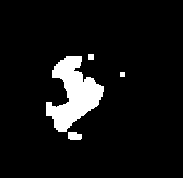
\includegraphics{threshold.png}
    \caption{Points corresponding to a ball in the image, separated via color range thresholding.}
    \label{fig:threshold}
\end{figure}

\subsection{Morphological Denoising and Outlier Rejection}

After background subtraction and thresholding are complete, extraneous noise pixels are removed through two additional methods. First, the image is eroded then dilated: an operation is first performed that shrinks white pixel shapes by setting every pixel to the minimum value in its neighborhood for a number of iterations, then the opposite effect is applied, wherein white pixel shapes are expanded multiple times by setting every pixel to the maximum value in its neighborhood. This causes small bits of noise to erode away entirely, and they don't return during the dilation step.

Subsequently, an outlier rejection algorithm is applied, whereby the mean position of all of the pixels is found, and any pixels that fall outside of two standard deviations of the mean are discarded. This removes any extraneous pixel groups that are far from the central grouping of pixels. It should be noted that this technique can have deleterious effects to object isolation if there are multiple meaningful pixel clusters at this point, which would occur if more than one ball has the same color. In those situations, it is better to avoid application of this technique. It should also be noted that outlier rejection incurs a major time penalty, and it seems a likely candidate for exclusion for performance-driven or real-time applications.

A post-denoising sample image is shown in Fig.~\ref{fig:denoised}.

\begin{figure}
\centering
    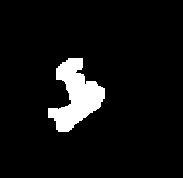
\includegraphics{denoised.png}
    \caption{Thresholded points corresponding to a ball in the image, after morphological denoising.}
    \label{fig:denoised}
\end{figure}

\subsection{Clustering for Center Determination}

After all of the aforementioned techniques have been applied, the remaining pixels should be clusters of points that are at least located on the balls, if not necessarily equivalent to all of their pixels. There should be one cluster corresponding to each ball. (Typically, it seems most effective to isolate ball colors at the thresholding step, but if there are multiple balls of the same color, there will be multiple groups of clusters at this step.)

K-means clustering is applied in order to find the centers of these clusters, and these centers are considered to be the positions of the balls. In practice, this often ends up being slightly inaccurate, as the spherical shape of the balls and non-uniform lighting in the scene usually results in shading that colors each ball differently on either side, and causes uneven object isolation. This causes k-means cluster centers to be displaced towards the side of greater recognition (usually, of greater color brightness). There are various techniques that may be able to be used to counteract this effect: future work could include refinement of these cluster centers using outlier rejection on the clusters before the application of a minimum enclosing circle on the remaining pixels.

After clustering, the observed positions are determined and can be drawn onto the original source image. A sample image of this is shown in Fig.~\ref{fig:clusters}.

\begin{figure}
\centering
    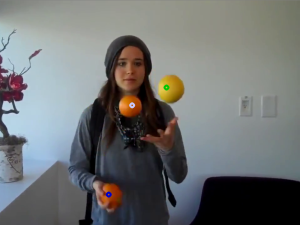
\includegraphics{clusters.png}
    \caption{Balls in the image are marked with observed positions based on k-means clustering.}
    \label{fig:clusters}
\end{figure}

\subsection{Optical Flow Estimation for Matching}

One vision-related problem still remains, which a careful reader may have already anticipated: if two balls are the same color and have been divided into two colors, the problem emerges of tracking each one independently between frames while maintaining a consistent identity. In other words, if there are two orange balls, which one is which across two subsequent frames?

Techniques from the field of optical flow estimation can be utilized to inform these decisions. In this implementation, the positions of all balls are maintained between frames, and at each new frame, a least-squares estimate is made in 4-dimensional velocity and position space in order to estimate which ball is which. The matching that results in the smallest squared velocity and position change is the one that will be used. More information about this technique, and others, can be found in \cite{fleet}.

Two consecutive frames, where markers show ball identities being maintained across frame boundaries, are shown in Fig.~ \ref{fig:matching}.

\begin{figure}
\centering
    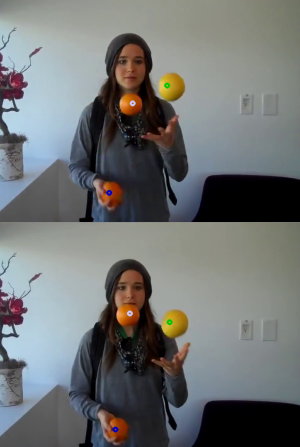
\includegraphics{matching.png}
    \caption{Two consecutive video frames illustrating how similarly colored balls are tracked independently (note the colors of the markers on the balls).}
    \label{fig:matching}
\end{figure}

%%%%%%%%%%%%%%%%%%%%%%%%%%%%%%%%%%%%%%%%%%%%%%%%%%%%%%%%%%%%%%%%%%%%%%%%%%%%%%%%
\section{STATE ESTIMATION}

After computer vision techniques have been applied to isolate the ``ball pixels," state estimation techniques can be applied to determine the position and velocitiy of each ball, and to predict their future states as well.

\subsection{Position and Velocity Observation}

As discussed above, the observed positions of each ball are determined after the application of k-means clustering. Their observed velocities can be determined by comparing these positions with positions estimated in the previous time step.

\subsection{Position and Velocity Prediction}

In addition to our observed values, predictions can be made for the position and velocity for the current time step using the previous state estimate and a knowledge of the system dynamics. When in mid-air, the only significant force affecting the balls should be the force due to gravity, which will cause an acceleration of approx. 9.81 m/s$^{2}$ in the negative vertical direction. The velocity of the balls should change based on this acceleration, while the position of the balls changes based on the velocity. Thus, by multiplying the calculated velocity by the timestep and adding to the previous position, we can get the current position, and similarly with the velocity:

\[
x_{k} = x_{k-1} + \dot{x}_{k-1} \Delta t \\ \\
\]
\[
\dot{x}_{k} = \dot{x}_{k-1} + \ddot{x}_{k-1} \Delta t
\]
\[
\ddot{x}_{k} = (0, -9.81) \text{ m/s}
\]

The astute reader may have already noticed that these predictions require a knowledge of the acceleration due to gravity in terms of screen pixels. This can be determined by calculating a mapping from pixel space to real-world space. For the purposes of this project, ``pixels per meter" calculations were determined by hand; however, it would be possible to empirically determine this information during a first pass on the video data by observing the acceleration of the balls within pixel space.

\subsection{Filtering for State Estimation}

Although significantly filtering was already performed during the ball isolation steps, the system is still subject to noise from incorrect position estimates and from the wholly unanticipated impulses applied to the balls whenever touched by the juggling. It is possible, however, to smooth this noise with state estimations that incorporate a filter based on the predicted state and the observed one. These techniques were applied to the states discussed above, resulting in somewhat smoother state estimates (but in some artifacts, which are discussed in the ``Results" section.)

\subsection{Trajectory Prediction}

In addition to a state estimate determination, a prediction of the future states of each ball can be made using similar techiques to those described in ``Position and Velocity Prediction" above. The states of the balls are propagated forward in time using Euler's method, and are then shown on the screen to visualize the future trajectory of the ball. A sample image of this is shown in Fig.~\ref{fig:trajectories}.

\begin{figure}
\centering
    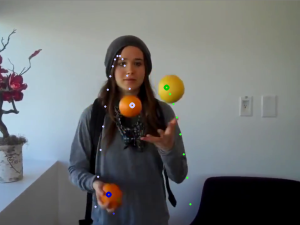
\includegraphics{trajectories.png}
    \caption{Trajectories of the balls are drawn using Euler's method to propagate their estimated states forward in time.}
    \label{fig:trajectories}
\end{figure}

%%%%%%%%%%%%%%%%%%%%%%%%%%%%%%%%%%%%%%%%%%%%%%%%%%%%%%%%%%%%%%%%%%%%%%%%%%%%%%%%
\section{RESULTS}

Various statement estimation techniques were attempted to perform the tracking task, with varying degrees of accuracy. Trials were run across multiple videos with differing lighting conditions, scales, and ball colors. Though most of the work was done based on pre-recorded videos, application to real-time video was also demonstrated.

\subsection{Observed States}

When the observed states were used directly as the estimated states of the balls, the result was surprisingly good; though significant error was visible with a thorough examination of the data being played in slow-motion, this error was not distracting and, to the eye, the tracking was rather good. (Due to time constraints, quantitative results for accuracy have yet to be obtained.)

A simple smoothing technique was performed by averaging observed velocity across timesteps, which resulted in a surprisingly smooth 

\subsection{Weighted State Combination}

A slightly more complicated technique was that of using a weighted combination of observed and predicted states, as with a constant-gain Kalman filter. This allowed adaptability and ``tweaking" to alter tracking accuracy. Slightly better results, with results more robust to tracking, were obtained with this technique.Weights that favored instantaneous observations were favored, probably due to integral error of slightly erroneous state estimations causing a high prediction weight to have a hard time converging on the correct state. Prediction accuracy seemed to vary often depending on the variables that are difficult to quantify, such as amount of spin on non-homogeneous balls, lighting in the room, length of time that balls were held, and other factors.

Equal weights for both instantaneous velocity observations and position observations were used, perhaps resulting in a larger degree of error than if the weights had been based on error covariances.

\subsection{Kalman Filtering}

 The Kalman filter incorporates both of these state determinations to build a (hopefully) more accurate state estimate, wherein the gains on each type of state determination are based on the changing state estimate covariance. However, full Kalman filtering was not used for this project, due to issues with quantifying process and measurement covariance accurately. Further work could attempt to adequately quantify these covariances in order to filter the data accurately enough to obtain satisfactory covergence properties.

%%%%%%%%%%%%%%%%%%%%%%%%%%%%%%%%%%%%%%%%%%%%%%%%%%%%%%%%%%%%%%%%%%%%%%%%%%%%%%%%
\section{CONCLUSIONS}

This project demonstrated how the application of a number of computer vision techniques, combined with control-theoretic state estimation techniques, can result in a robust (and visually pleasing) system for tracking the movement of balls in a video scene. There is much room for improvement: it would be of great interest to remove the need to manually specify color ranges for balls, and many improvements could be made (as discussed earlier) to obtain more accurate observations for ball centers. Additionally, proper quantification of error covariances to allow varying Kalman gains could be very beneficial to tracking accuracy. However, the results as obtained are still satisfactory and seem promising for future applications.

%%%%%%%%%%%%%%%%%%%%%%%%%%%%%%%%%%%%%%%%%%%%%%%%%%%%%%%%%%%%%%%%%%%%%%%%%%%%%%%%
\section{ACKNOWLEDGMENTS}

The author gratefully acknowledges the help and tutelage of the course professor, Dr. Kristi Morgansen, and the teaching assistant, Jake Quenzer. Computer vision advice obtained in conversations with Dr. Brian Curless was also very valuable to the completion of this project.

%%%%%%%%%%%%%%%%%%%%%%%%%%%%%%%%%%%%%%%%%%%%%%%%%%%%%%%%%%%%%%%%%%%%%%%%%%%%%%%%

\begin{thebibliography}{99}

\bibitem{kalmanapollo}
Grewal, M.S., Andrews, A.P., ``Applications of Kalman Filtering in Aerospace 1960 to the Present," IEEE Control Systems Magazine 30(3), 69-78 (2010).

\bibitem{funk}
Funk, N., ``A Study of the Kalman Filter Applied to Visual Tracking." University of Alberta, 2003.

\bibitem{hough}
Hough, P. V. C., ``Methods and Means for Recognizing Complex Patterns," U.S. Patent 3069654, 1962.

\bibitem{fleet}
Fleet, D., Weiss, Y., ``Optical Flow Estimation" (from Mathematical models for Computer Vision: The Handbook), Springer,m pp. 239-257, 2005.

\bibitem{zoran1}
Zivkovic, Z., van der Heijden, F., ``Efficient adaptive density estimation per image pixel for the task of background subtraction," Pattern Recogn. Lett. 27, 7, 773-780, 2006.

\bibitem{zoran2}
Zivkovic, Z., ``Improved adaptive Gaussian mixture model for background subtraction," Pattern Recognition, 2004. ICPR 2004. Proceedings of the 17th International Conference on, vol.2, no., pp.28,31 Vol.2, 23-26 Aug. 2004.

\end{thebibliography}

\end{document}
